\documentclass[a4paper]{article}
\usepackage[utf8]{inputenc}
\usepackage[english]{babel}
\usepackage{indentfirst}
\usepackage[a4paper, top = 1.5cm, bottom=1.5cm,left=2cm,right=1cm]{geometry}
\usepackage{amsmath}
\usepackage{amsfonts}
\usepackage{graphicx}
\usepackage{wrapfig}
\usepackage{hyperref}


\usepackage[linesnumbered,ruled,vlined]{algorithm2e}

\setlength{\parindent}{0.1ex}
\setlength{\parskip}{1em}

\title{Numerical Integration}
\author{Nikita Sattarov, 322 gr.}
\date{October 2020}


\SetCommentSty{mycommfont}


\begin{document}
\maketitle
%\newcommand{\anonsection}[1]{\section*{#1}\addcontentsline{toc}{section}{#1}}
%\newcommand{\anonsubsection}[1]{\subsection*{#1}\addcontentsline{toc}{subsection}{#1}}
%\newcommand{\anonsubsubsection}[1]{\subsubsection*{#1}\addcontentsline{toc}{subsubsection}{#1}}
\newcommand{\ds}{\displaystyle}


\begin{wrapfigure}{r}{0.25\textwidth}
	\begin{center}
		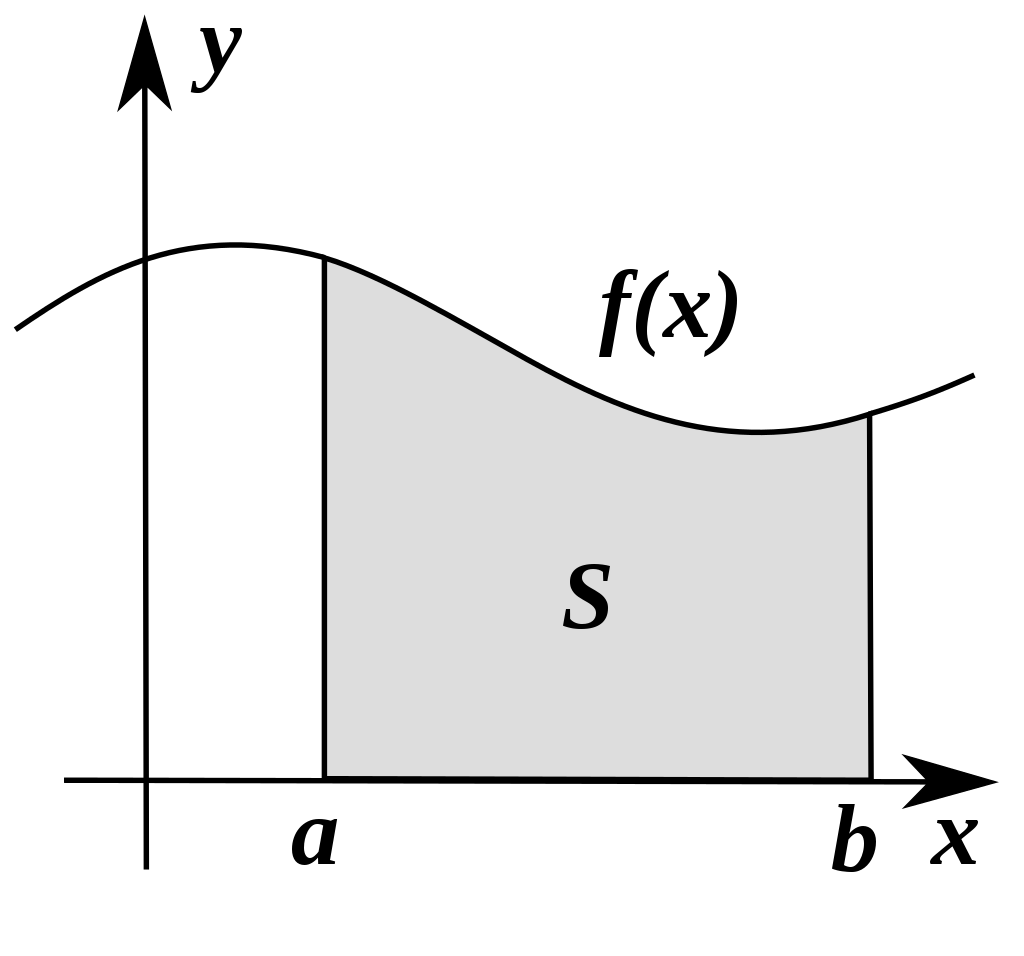
\includegraphics[width=0.2\textwidth]{1}
	\end{center}
	\caption{Numerical integration is used to calculate a numerical approximation for the value ${\ds S}$, the area under the curve defined by ${\ds f(x)}$.}
\end{wrapfigure}
In analysis, \textbf{numerical integration} comprises a broad family of algorithms for calculating the numerical value of a definite integral, and by extension, the term is also sometimes used to describe the numerical solution of differential equations. This article focuses on calculation of definite integrals. The term \textbf{numerical quadrature} (often abbreviated to \textit{quadrature}) is more or less a synonym for \textit{numerical integration}, especially as applied to one-dimensional integrals. Some authors refer to numerical integration over more than one dimension as \textbf{cubature};$^{~\cite{weisstein2000cubature}}$ others take \textit{quadrature} to include higher-dimensional integration.

The basic problem in numerical integration is to compute an approximate solution to a definite integral

\begin{equation*}
	\int _{a}^{b}f(x)\,dx
\end{equation*}

to a given degree of accuracy. If $f(x)$ is a smooth function integrated over a small number of dimensions, and the domain of integration is bounded, there are many methods for approximating the integral to the desired precision.

\tableofcontents

\section{History}
The term "numerical integration" first appears in 1915 in the publication \textit{A Course in Interpolation and Numeric Integration for the Mathematical Laboratory} by David Gibb.$^{~\cite{miller2015earliest}}$

\textbf{Quadrature} is a historical mathematical term that means calculating area. Quadrature problems have served as one of the main sources of mathematical analysis. Mathematicians of Ancient Greece, according to the Pythagorean doctrine, understood calculation of area as the process of constructing geometrically a square having the same area (\textit{squaring}). That is why the process was named \textbf{quadrature}. For example, a quadrature of the circle, Lune of Hippocrates, The Quadrature of the Parabola. This construction must be performed only by means of compass and straightedge.

The ancient Babylonians used the trapezoidal rule to integrate the motion of Jupiter along the ecliptic.$^{~\cite{ossendrijver2016ancient}}$

\begin{wrapfigure}{l}{0.2\textwidth}
	\begin{center}
		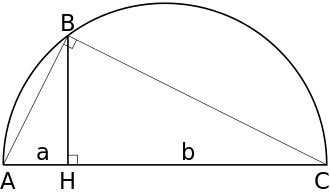
\includegraphics[width=0.2\textwidth]{2}
	\end{center}
	\caption{Antique method to find the Geometric mean}
\end{wrapfigure}
For a quadrature of a rectangle with the sides $a$ and $b$ it is necessary to construct a square with the side ${\ds x={\sqrt {ab}}}$ (the Geometric mean of $a$ and $b$). For this purpose it is possible to use the following fact: if we draw the circle with the sum of $a$ and $b$ as the diameter, then the height BH (from a point of their connection to crossing with a circle) equals their geometric mean. The similar geometrical construction solves a problem of a quadrature for a parallelogram and a triangle.

Problems of quadrature for curvilinear figures are much more difficult. The quadrature of the circle with compass and straightedge had been proved in the 19th century to be impossible. Nevertheless, for some figures (for example the Lune of Hippocrates) a quadrature can be performed. The quadratures of a sphere surface and a parabola segment done by Archimedes became the highest achievement of the antique analysis.

\begin{itemize}
\item The area of the surface of a sphere is equal to quadruple the area of a great circle of this sphere.
\item The area of a segment of the parabola cut from it by a straight line is 4/3 the area of the triangle inscribed in this segment.
\end{itemize}

\begin{wrapfigure}{r}{0.2\textwidth}
	\begin{center}
		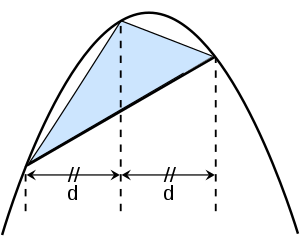
\includegraphics[width=0.2\textwidth]{3}
	\end{center}
	\caption{The area of a segment of a parabola}
\end{wrapfigure}
For the proof of the results Archimedes used the Method of exhaustion of Eudoxus.

In medieval Europe the quadrature meant calculation of area by any method. More often the Method of indivisibles was used; it was less rigorous, but more simple and powerful. With its help Galileo Galilei and Gilles de Roberval found the area of a cycloid arch, Gr\'egoire de Saint-Vincent investigated the area under a hyperbola (\textit{Opus Geometricum}, 1647), and Alphonse Antonio de Sarasa, de Saint-Vincent's pupil and commentator, noted the relation of this area to logarithms.

John Wallis algebrised this method: he wrote in his \textit{Arithmetica Infinitorum} (1656) series that we now call the definite integral, and he calculated their values. Isaac Barrow and James Gregory made further progress: quadratures for some algebraic curves and spirals. Christiaan Huygens successfully performed a quadrature of some Solids of revolution.

The quadrature of the hyperbola by Saint-Vincent and de Sarasa provided a new function, the natural logarithm, of critical importance.

With the invention of integral calculus came a universal method for area calculation. In response, the term \textbf{quadrature} has become traditional, and instead the modern phrase "\textit{computation of a univariate definite integral}" is more common.

\section{Reasons for numerical integration}
There are several reasons for carrying out numerical integration.

\begin{enumerate}
\item The integrand $f(x)$ may be known only at certain points, such as obtained by sampling. Some embedded systems and other computer applications may need numerical integration for this reason.
\item A formula for the integrand may be known, but it may be difficult or impossible to find an antiderivative that is an elementary function. An example of such an integrand is $f(x) = exp \left( -x^2 \right)$, the antiderivative of which (the error function, times a constant) cannot be written in elementary form.
\item It may be possible to find an antiderivative symbolically, but it may be easier to compute a numerical approximation than to compute the antiderivative. That may be the case if the antiderivative is given as an infinite series or product, or if its evaluation requires a special function that is not available.
\end{enumerate}

\section{Methods for one-dimensional integrals}
Numerical integration methods can generally be described as combining evaluations of the integrand to get an approximation to the integral. The integrand is evaluated at a finite set of points called \textbf{integration points} and a weighted sum of these values is used to approximate the integral. The integration points and weights depend on the specific method used and the accuracy required from the approximation.

An important part of the analysis of any numerical integration method is to study the behavior of the approximation error as a function of the number of integrand evaluations. A method that yields a small error for a small number of evaluations is usually considered superior. Reducing the number of evaluations of the integrand reduces the number of arithmetic operations involved, and therefore reduces the total round-off error. Also, each evaluation takes time, and the integrand may be arbitrarily complicated.

A 'brute force' kind of numerical integration can be done, if the integrand is reasonably well-behaved (i.e. piecewise continuous and of bounded variation), by evaluating the integrand with very small increments.

\subsection{Quadrature rules based on interpolating functions}
A large class of quadrature rules can be derived by constructing interpolating functions that are easy to integrate. Typically these interpolating functions are polynomials. In practice, since polynomials of very high degree tend to oscillate wildly, only polynomials of low degree are used, typically linear and quadratic.

\begin{wrapfigure}{r}{0.2\textwidth}
	\begin{center}
		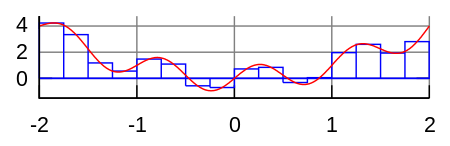
\includegraphics[width=0.2\textwidth]{4}
	\end{center}
	\caption{Illustration of the rectangle rule.}
\end{wrapfigure}

The simplest method of this type is to let the interpolating function be a constant function (a polynomial of degree zero) that passes through the point $\left({\frac {a+b}{2}},f\left({\frac {a+b}{2}}\right)\right)$. This is called the \textit{midpoint rule} or \textit{rectangle rule}

\begin{equation*}
	\int _{a}^{b}f(x)\,dx\approx (b-a)f\left({\frac {a+b}{2}}\right).
\end{equation*}

\begin{wrapfigure}{r}{0.2\textwidth}
	\begin{center}
		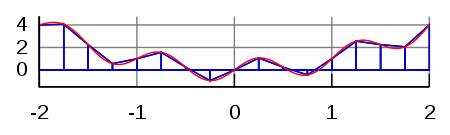
\includegraphics[width=0.2\textwidth]{5}
	\end{center}
	\caption{Illustration of the trapezoidal rule.}
\end{wrapfigure}

The interpolating function may be a straight line (an affine function, i.e. a polynomial of degree 1) passing through the points ${\ds \left(a,f(a)\right)}$ and ${\ds \left(b,f(b)\right)}$. This is called the \textit{trapezoidal rule}

\begin{equation*}
	\int _{a}^{b}f(x)\,dx\approx (b-a)\left({\frac {f(a)+f(b)}{2}}\right).
\end{equation*}

\begin{wrapfigure}{r}{0.2\textwidth}
	\begin{center}
		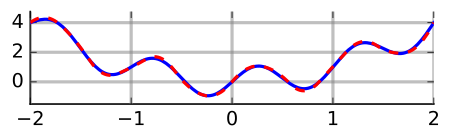
\includegraphics[width=0.2\textwidth]{6}
	\end{center}
	\caption{Illustration of Simpson's rule.}
\end{wrapfigure}

For either one of these rules, we can make a more accurate approximation by breaking up the interval ${\ds [a,b]}$  into some number $n$ of subintervals, computing an approximation for each subinterval, then adding up all the results. This is called a \textit{composite rule}, \textit{extended rule}, or \textit{iterated rule}. For example, the composite trapezoidal rule can be stated as

\begin{equation*}
	\int _{a}^{b}f(x)\,dx\approx {\frac {b-a}{n}}\left({f(a) \over 2}+\sum _{k=1}^{n-1}\left(f\left(a+k{\frac {b-a}{n}}\right)\right)+{f(b) \over 2}\right),
\end{equation*}

where the subintervals have the form ${\ds [a+kh,a+(k+1)h]\subset [a,b],}$ with $h={\frac {b-a}{n}}$ and ${\ds k=0,\ldots ,n-1.}$ Here we used subintervals of the same length $h$ but one could also use intervals of varying length ${\ds \left(h_{k}\right)_{k}}$.

Interpolation with polynomials evaluated at equally spaced points in ${\ds [a,b]}$ yields the Newton–Cotes formulas, of which the rectangle rule and the trapezoidal rule are examples. Simpson's rule, which is based on a polynomial of order 2, is also a Newton–Cotes formula.

Quadrature rules with equally spaced points have the very convenient property of \textit{nesting}. The corresponding rule with each interval subdivided includes all the current points, so those integrand values can be re-used.

If we allow the intervals between interpolation points to vary, we find another group of quadrature formulas, such as the Gaussian quadrature formulas. A Gaussian quadrature rule is typically more accurate than a Newton–Cotes rule, which requires the same number of function evaluations, if the integrand is smooth (i.e., if it is sufficiently differentiable). Other quadrature methods with varying intervals include Clenshaw–Curtis quadrature (also called Fej\'er quadrature) methods, which do nest.

Gaussian quadrature rules do not nest, but the related Gauss–Kronrod quadrature formulas do.

\subsection{Generalized midpoint rule formula}
A generalized midpoint rule formula is given by

\begin{equation*}
	\int _{0}^{1}{f(x)\,dx}=\sum _{m=1}^{M}{\sum _{n=0}^{\infty }{{\frac {{{\left({-1}\right)}^{n}}+1}{{{\left({2M}\right)}^{n+1}}\left({n+1}\right)!}}{{\left.{{f^{\left(n\right)}}\left(x\right)}\right|}_{x={\frac {m-1/2}{M}}}}}}
\end{equation*}

or

\begin{equation*}
	\int _{0}^{1}{f(x)\,dx}=\lim _{M\to \infty }\sum _{m=1}^{M}{\sum _{n=0}^{N}{{\frac {{{\left({-1}\right)}^{n}}+1}{{{\left({2M}\right)}^{n+1}}\left({n+1}\right)!}}{{\left.{{f^{\left(n\right)}}\left(x\right)}\right|}_{x={\frac {m-1/2}{M}}}}}},
\end{equation*}

where ${\ds f^{(n)}(x)}$ denotes $n$-th derivative. For example, substituting ${\ds M=1}$ and

\begin{equation*}
	f(x)={\frac {\theta }{1+\theta ^{2}x^{2}}}
\end{equation*}

in the generalized midpoint rule formula, we obtain an equation of the inverse tangent
\begin{equation*}
	\tan ^{-1}(\theta )=i\sum _{n=1}^{\infty }{\frac {1}{2n-1}}\left({\frac {1}{\left(1+2i/\theta \right)^{2n-1}}}-{\frac {1}{\left(1-2i/\theta \right)^{2n-1}}}\right)=2\sum _{n=1}^{\infty }{{\frac {1}{2n-1}}{\frac {{{a}_{n}}\left(\theta \right)}{a_{n}^{2}\left(\theta \right)+b_{n}^{2}\left(\theta \right)}}},
\end{equation*}

where ${\ds i={\sqrt {-1}}}$ is imaginary unit and

\begin{equation*}
	\begin{aligned}
		a_{1}(\theta )&={\frac {2}{\theta }},\\
		b_{1}(\theta )&=1,\\
		a_{n}(\theta )&=\left(1-{\frac {4}{\theta ^{2}}}\right)\,a_{n-1}(\theta )+{\frac {4}{\theta }}\,b_{n-1}(\theta ),\\
		b_{n}(\theta )&=\left(1-{\frac {4}{\theta ^{2}}}\right)\,b_{n-1}(\theta )-{\frac {4}{\theta }}\,a_{n-1}(\theta ).
	\end{aligned}
\end{equation*}

Since at each odd $n$ the numerator of the integrand becomes ${\ds (-1)^{n}+1=0}$, the generalized midpoint rule formula can be reorganized as

\begin{equation*}
	\int _{0}^{1}{f(x)\,dx}=2\sum _{m=1}^{M}{\sum _{n=0}^{\infty }{{\frac {1}{{{\left({2M}\right)}^{2n+1}}\left({2n+1}\right)!}}{{\left.{{f^{(2n)}}(x)}\right|}_{x={\frac {m-1/2}{M}}}}}}\,\,.
\end{equation*}

The following example of Mathematica code generates the plot showing difference between inverse tangent and its approximation truncated at ${\ds M=5}$ and ${\ds N=10}$:

\begin{algorithm}[H]
$f[theta\_, x\_] := theta/(1 + theta^2*x^2)$\;
$aTan[theta\_, M\_, nMax\_] := 
    2*Sum[(Function[x, Evaluate[D[f[theta, x], {x, 2*n}]]][(m - 1/2)/
        M])/((2*n + 1)!*(2*M)^{(2*n + 1)}), {m, 1, M}, {n, 0, nMax}]$\;
$Plot[{ArcTan[theta] - aTan[theta, 5, 10]}, {theta, -Pi, Pi}, 
 PlotRange \rightarrow All]$\;
\end{algorithm}

For a function ${\ds g(t)}$  defined over interval ${\ds (a,b)}$, its integral is

\begin{equation*}
	\int _{a}^{b}{g(t)dt}=\int _{0}^{b-a}{g(\tau +a)d\tau }=(b-a)\int _{0}^{1}{g((b-a)x+a)\,dx}.
\end{equation*}

Therefore, we can apply the generalized midpoint integration formula above by assuming that ${\ds f(x)=(b-a)\,g((b-a)x+a)}$.

\subsection{Adaptive algorithms}
If $f(x)$ does not have many derivatives at all points, or if the derivatives become large, then Gaussian quadrature is often insufficient. In this case, an algorithm similar to the following will perform better:

\begin{algorithm}[H]

  \DontPrintSemicolon

  \SetKwFunction{FCalc}{$calculate\_definite\_integral\_of\_f$}

  \SetKwProg{Fn}{Def}{:}{}
  \SetKwProg{FWhile}{While}{:}{}
  \SetKwProg{FIf}{If}{:}{}
  \SetKwProg{FElse}{Else}{:}{}
  \Fn{\FCalc{$f$, $initial\_step\_size$}}{
        ''''''\;
        This algorithm calculates the definite integral of a function from 0 to 1, adaptevily, by choosing smaller steps near problematic points.\;
        ''''''\;
        x = 0.0\;
        h = initial\_step\_size\;
        accumulator = 0.0\;
      	\FWhile{{$x < 1.0$}}{
        	\FIf{{$x + h > 1.0$}}{
        		h = 1.0 - x    $\#$At end of unit interval, adjust last step to end at 1.\;
        	}
        	\FIf{{error\_too\_big\_in\_quadrature\_of\_f\_over\_range(f, [x, x + h])}}{
        		h = make\_h\_smaller(h)\;
		}
		\FElse{{$ $}}{
			accumulator += quadrature\_of\_f\_over\_range(f, [x, x + h])\;
			x += h\;
			\FIf{{error\_too\_small\_in\_quadrature\_of\_over\_range(f, [x, x + h])}}{
				h = make\_h\_larger(h) $\#$Avoid wasting time on tiny steps.
			}
		}
	}
        \KwRet accumulator\;
  }
\end{algorithm}

Some details of the algorithm require careful thought. For many cases, estimating the error from quadrature over an interval for a function $f(x)$ isn't obvious. One popular solution is to use two different rules of quadrature, and use their difference as an estimate of the error from quadrature. The other problem is deciding what "too large" or "very small" signify. A \textit{local} criterion for "too large" is that the quadrature error should not be larger than $t \cdot h$ where $t$, a real number, is the tolerance we wish to set for global error. Then again, if $h$ is already tiny, it may not be worthwhile to make it even smaller even if the quadrature error is apparently large. A \textit{global} criterion is that the sum of errors on all the intervals should be less than $t$. This type of error analysis is usually called "a posteriori" since we compute the error after having computed the approximation.

Heuristics for adaptive quadrature are discussed by Forsythe et al.

\subsection{Extrapolation methods}
The accuracy of a quadrature rule of the Newton-Cotes type is generally a function of the number of evaluation points. The result is usually more accurate as the number of evaluation points increases, or, equivalently, as the width of the step size between the points decreases. It is natural to ask what the result would be if the step size were allowed to approach zero. This can be answered by extrapolating the result from two or more nonzero step sizes, using series acceleration methods such as Richardson extrapolation. The extrapolation function may be a polynomial or rational function. Extrapolation methods are described in more detail by Stoer and Bulirsch and are implemented in many of the routines in the QUADPACK library.

\subsection{Conservative (a priori) error estimation}
Let $f$ have a bounded first derivative over ${\ds [a,b],}$ i.e. ${\ds f\in C^{1}([a,b])}$. The mean value theorem for $f$, where ${\ds x\in [a,b),}$ gives

\begin{equation*}
	(x-a)f'(\xi _{x})=f(x)-f(a),
\end{equation*}

for some ${\ds \xi _{x}\in (a,x]}$ depending on $x$.

If we integrate in $x$ from $a$ to $b$ on both sides and take the absolute values, we obtain

\begin{equation*}
	\left|\int _{a}^{b}f(x)\,dx-(b-a)f(a)\right|=\left|\int _{a}^{b}(x-a)f'(\xi _{x})\,dx\right|.
\end{equation*}

We can further approximate the integral on the right-hand side by bringing the absolute value into the integrand, and replacing the term in ${\ds f'}$ by an upper bound

\begin{equation*}
	\left|\int _{a}^{b}f(x)\,dx-(b-a)f(a)\right|\leq {(b-a)^{2} \over 2}\sup _{a\leq x\leq b}\left|f'(x)\right|,
\end{equation*}

where the supremum was used to approximate.

Hence, if we approximate the integral $ \int _{a}^{b}f(x)\,dx$ by the quadrature rule ${\ds (b-a)f(a)}$ our error is no greater than the right hand side of $1$. We can convert this into an error analysis for the Riemann sum (*), giving an upper bound of

\begin{equation*}
	{n^{-1} \over 2}\sup _{0\leq x\leq 1}\left|f'(x)\right|
\end{equation*}

for the error term of that particular approximation. (Note that this is precisely the error we calculated for the example ${\ds f(x)=x}$). Using more derivatives, and by tweaking the quadrature, we can do a similar error analysis using a Taylor series (using a partial sum with remainder term) for $f$. This error analysis gives a strict upper bound on the error, if the derivatives of $f$ are available.

This integration method can be combined with interval arithmetic to produce computer proofs and \textit{verified} calculations.

\subsection{Integrals over infinite intervals}

Several methods exist for approximate integration over unbounded intervals. The standard technique involves specially derived quadrature rules, such as Gauss-Hermite quadrature for integrals on the whole real line and Gauss-Laguerre quadrature for integrals on the positive reals.$^{~\cite{leader2004numerical}}$ Monte Carlo methods can also be used, or a change of variables to a finite interval; e.g., for the whole line one could use

\begin{equation*}
	\int _{-\infty }^{\infty }f(x)\,dx=\int _{-1}^{+1}f\left({\frac {t}{1-t^{2}}}\right){\frac {1+t^{2}}{(1-t^{2})^{2}}}\,dt,
\end{equation*}

and for semi-infinite intervals one could use

\begin{equation*}
	\begin{aligned}
		\int _{a}^{\infty }f(x)\,dx&=\int _{0}^{1}f\left(a+{\frac {t}{1-t}}\right){\frac {dt}{(1-t)^{2}}},\\
		\int _{-\infty }^{a}f(x)\,dx&=\int _{0}^{1}f\left(a-{\frac {1-t}{t}}\right){\frac {dt}{t^{2}}},
	\end{aligned}
\end{equation*}

as possible transformations.

\section{Multidimensional integrals}
The quadrature rules discussed so far are all designed to compute one-dimensional integrals. To compute integrals in multiple dimensions, one approach is to phrase the multiple integral as repeated one-dimensional integrals by applying Fubini's theorem (the tensor product rule). This approach requires the function evaluations to grow exponentially as the number of dimensions increases. Three methods are known to overcome this so-called \textit{curse of dimensionality}.

A great many additional techniques for forming multidimensional cubature integration rules for a variety of weighting functions are given in the monograph by Stroud.$^{~\cite{stroud1971approximate}}$

\subsection{Monte Carlo}
Monte Carlo methods and quasi-Monte Carlo methods are easy to apply to multi-dimensional integrals. They may yield greater accuracy for the same number of function evaluations than repeated integrations using one-dimensional methods.$^{[citation \, \, \, needed]}$

A large class of useful Monte Carlo methods are the so-called Markov chain Monte Carlo algorithms, which include the Metropolis-Hastings algorithm and Gibbs sampling.

\subsection{Sparse grids}
Sparse grids were originally developed by Smolyak for the quadrature of high-dimensional functions. The method is always based on a one-dimensional quadrature rule, but performs a more sophisticated combination of univariate results. However, whereas the tensor product rule guarantees that the weights of all of the cubature points will be positive if the weights of the quadrature points were positive, Smolyak's rule does not guarantee that the weights will all be positive.

\subsection{Bayesian Quadrature}
Bayesian Quadrature is a statistical approach to the numerical problem of computing integrals and falls under the field of probabilistic numerics. It can provide a full handling of the uncertainty over the solution of the integral expressed as a Gaussian Process posterior variance. It is also known to provide very fast convergence rates which can be up to exponential in the number of quadrature points n.$^{~\cite{briol2015frank}}$

\section{Connection with differential equations}
The problem of evaluating the integral

\begin{equation*}
	F(x)=\int _{a}^{x}f(u)\,du
\end{equation*}

can be reduced to an initial value problem for an ordinary differential equation by applying the first part of the fundamental theorem of calculus. By differentiating both sides of the above with respect to the argument $x$, it is seen that the function $F$ satisfies

\begin{equation*}
	{\frac {dF(x)}{dx}}=f(x),\quad F(a)=0.
\end{equation*}

Methods developed for ordinary differential equations, such as Runge''--~Kutta methods, can be applied to the restated problem and thus be used to evaluate the integral. For instance, the standard fourth-order Runge''--~Kutta method applied to the differential equation yields Simpson's rule from above.

The differential equation ${\ds F'(x)=f(x)}$ has a special form: the right-hand side contains only the independent variable (here $x$) and not the dependent variable (here ${\ds F}$). This simplifies the theory and algorithms considerably. The problem of evaluating integrals is thus best studied in its own right.

\bibliographystyle{gost2008}
\nocite{barnhill1976philip}
\nocite{forsythe1977computer}
\nocite{press2007numerical}
\nocite{stoer2013introduction}
\nocite{boyer2011history}
\nocite{eves1990introduction}
\bibliography{biblio}


\end{document}